\documentclass[12pt]{exam}
\usepackage[utf8]{inputenc}

\usepackage[margin=1in]{geometry}
\usepackage{amsmath,amssymb}
\usepackage{multicol}
\usepackage{url}
\usepackage{graphicx}


\PassOptionsToPackage{hyphens}{url}\usepackage{hyperref}
\newcommand{\class}{Robot Intelligence}
\newcommand{\term}{Fall 2020}
\newcommand{\examnum}{MidTerm Exam}
\newcommand{\examdate}{9/6/2021}
\newcommand{\timelimit}{10/29/2021}

\pagestyle{head}
\firstpageheader{}{}{}
\runningheader{\class}{\examnum\ - Page \thepage\ of \numpages}{\examdate}
\runningheadrule


\begin{document}

\noindent
\begin{tabular*}{\textwidth}{l @{\extracolsep{\fill}} r @{\extracolsep{6pt}} l}
\textbf{\class} & \textbf{Name:} & \makebox[2in]{\hrulefill}\\
\textbf{\term} &&\\
\textbf{\examnum} &&\\
\textbf{\examdate} &&\\
\textbf{Take Home Exam - Due Before Class on Canvas \timelimit} 
\end{tabular*}\\
\rule[2ex]{\textwidth}{2pt}

This exam contains \numpages\ pages (including this cover page) and \numquestions\ questions.\\
Total number of points is \numpoints. Undergraduate students are required to answer 7 questions, graduate students must answer 9. Any additional questions answered will not only be counted as additional credits, but you will have a good feeling deep inside (probably). 

Any programming/code artifacts associated with this exam should be submitted along with the final PDF to canvas. Please put your entire submission in a single .zip file. 

This exam will cover topics in motion, planning, sensor processing, and ethics.


\begin{center}
Grade Table (Quick view to see the breakdown)\\
\addpoints
\gradetable[v][questions]
\end{center}

\noindent
\rule[2ex]{\textwidth}{2pt}

\begin{questions}

% \question[1] Calculate 2+2.
% \addpoints

% \question[5] Consider the function $f(x)=3x^3+2x^2+x+1$.
% \noaddpoints % to omit double points count
% \begin{parts}
% \part[10] Calculate $f'(x)$.
% \part[10] Calculate $f''(x)$.
% \end{parts}
% \addpoints

% \question[2] One of these things is not like the others; one of these
% things is not the same. Which one is different?
% \begin{choices}
% \choice John
% \choice Paul
% \choice George
% \choice Ringo
% \choice Socrates
% \end{choices}

% \question[2] One of these things is not like the others; one of these
% things is not the same. Which one is different?
% \begin{oneparchoices}
% \choice John
% \choice Paul
% \choice George
% \choice Ringo
% \choice Socrates
% \end{oneparchoices}

% \question[3] Mark box if true.
% \addpoints
% \begin{checkboxes}
% \choice 2+2=4
% \choice $\frac{d}{dx} (x^2+1) = 2x+1$
% \choice The Moon is made of cheese.
% \end{checkboxes}

% {%
% \checkboxchar{$\Box$} % changing checkbox style locally
% \question[3] Mark box if true.
% \addpoints
% \begin{checkboxes}
% \choice 2+2=4
% \choice $\frac{d}{dx} (x^2+1) = 2x+1$
% \choice The Moon is made of cheese.
% \end{checkboxes}
% }%

% {%
% % changing choice items style locally
% \renewcommand*\thechoice{\arabic{choice}} 
% \renewcommand*\choicelabel{\thechoice)}
% %
% \question[2] Element with $Z=92$ is:
% \begin{multicols}{2}
% \begin{choices}
% \choice H
% \choice O
% \choice F
% \choice S
% \choice Ba
% \choice Pb
% \choice U
% \choice Pu
% \end{choices}
% \end{multicols}
% }%

% \question[10]
% In no more than two sentences, explain the difference between RRT* and A*.
% % \makeemptybox{2in}

% \question[10]
% Write the psuedo code for the Djikstra's algorithm and explain how it searches a space and finds the optimal path
% % \makeemptybox{\fill}

% \question[10]
% Write the psuedo code for the RRT* algorithm and explain how the search can be  guided

% \question[15]
% \noaddpoints
% Understanding key algorithms
% \begin{parts}
% \part[5] List two unique features of the RRT*, A*, and Djikstra's algorithm
% \part[5] Which algorithm is best suited for an holonomic ground robot with few known obstacles? (Why? What are your assumptions?)
% \part[5] Which algorithm is best suited for navigation autonomy on a field combat tank? (Why? What are your assumptions?)
% \end{parts}

\newpage

\addpoints
\question[20]
Moving in a car

A $4.0m$ long car is making a right hand turn with a steering angle $\alpha = \frac{\pi}{6}$, it maintains a forward velocity of $20 m/s$. 
\noaddpoints
\begin{parts}
\part[5] Draw a diagram of the vehicle and write the discretized equations of motion for this vehicle's pose (x, y, $\theta$)
\part[5] Calculate the radius of curvature $R$ of this vehicle at the given steering angle
\part[10] If the car is traveling for $10s$, what is my position error using the discretized equations of motion if I define my time steps at $\Delta t = 1, 0.1, 0.01$ ? Plot the errors and computing time for these cases.
\end{parts}
% \fillwithlines{\fill}

\newpage

\addpoints
\question[20]
Balancing a Pole 

A cart and pole suddenly appears before you and you feel compelled to answer burning questions you have always held about these systems. 

\noaddpoints
\begin{parts}
\part[5] 
\begin{figure}
    \centering
    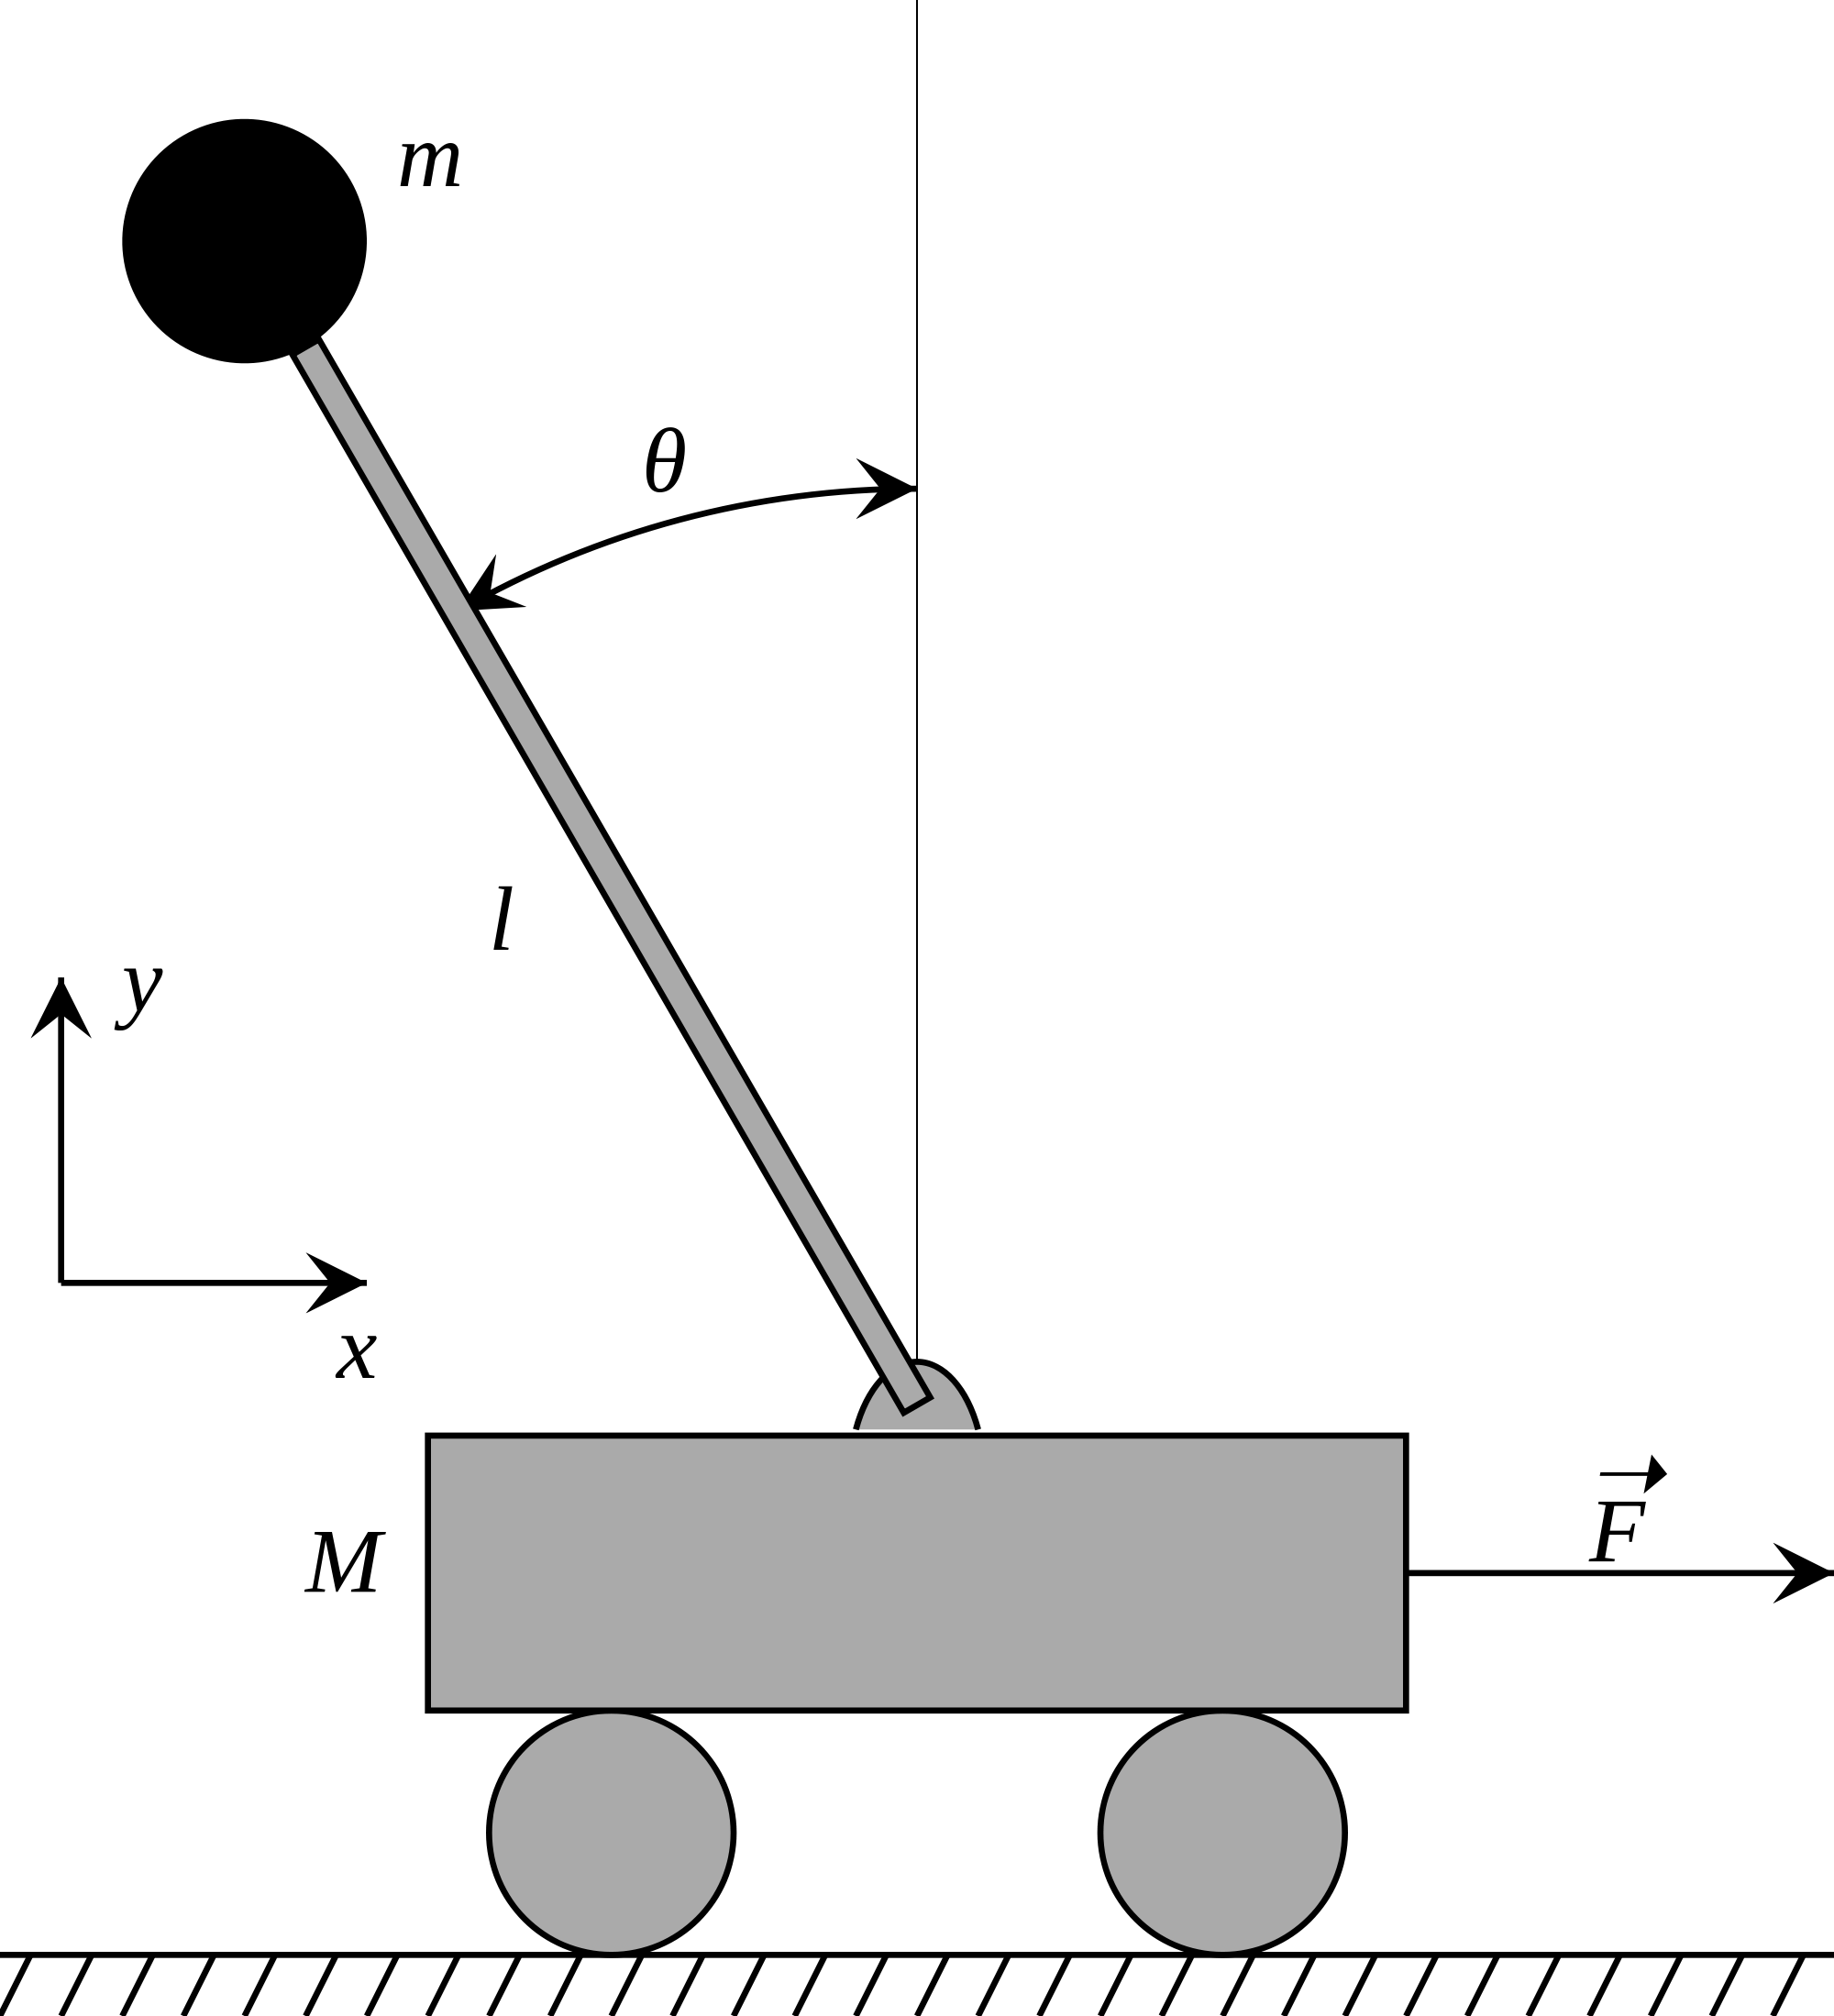
\includegraphics[width=0.5\textwidth]{cart-pole.png}
    \caption{Assume that the mass $m = 0.2kg$, $l = 1.0$, $M = 4.0kg$}
    \label{fig:cartpole}
\end{figure}
Describe the equations of motion that governs this system
\part[10] Generate code for a controller that would be able to keep the pole balanced in the air. 
\part[5] What is the maximum angle that my pole can fall to before it cannot recover if max Force $F = 6N $?
\end{parts}

\newpage

\addpoints
\question[20]

Control and Reinforcement Learning
\noaddpoints
\begin{parts}
\part[5] Explain three merits and three demerits of using reinforcement learning for mechatronic systems.
\part[5] Draw a diagram for reinforcement learning and controls and contrast the two
\part[10] Implement this example of a 2D running robot (cheetah)  \url{https://github.com/openai/gym/blob/master/gym/envs/mujoco/half_cheetah.py} and adapt the code to penalize hip motor movements faster than $\pi \frac{rad}{s}$

\end{parts}

% \newpage

% \addpoints
% \question[20]

% Robot Arms

% \noaddpoints
% \begin{parts}



% \part[5] 
% \begin{figure}
% \centering
% 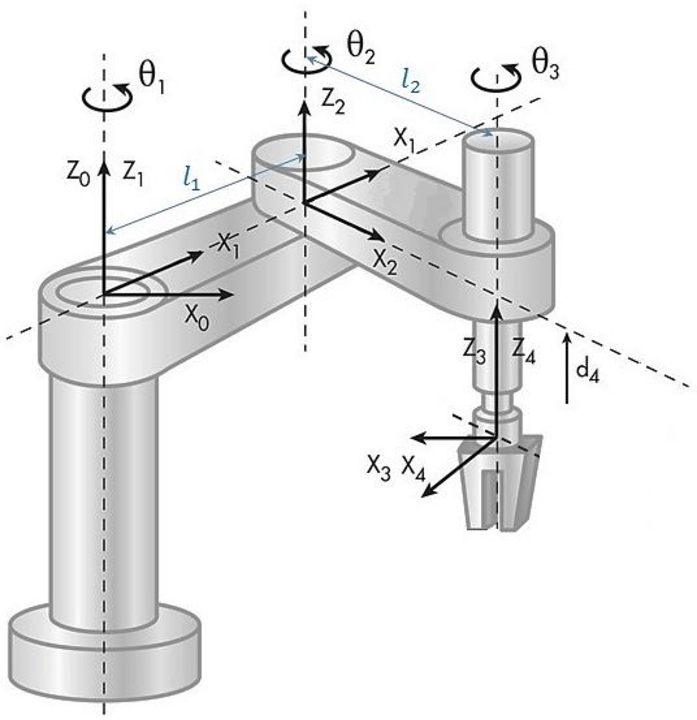
\includegraphics[width=0.5\textwidth]{SCARA-robot-of-4-gdl-Source-Our-elaboration.png}
% \caption{SCARA type manipulator. }
% \end{figure}

% What is the workspace volume for this robot?. (Draw a picture of it as well)
% \part[5] Write the DH parameters and forward kinematics for this robot 
% \part[10] Compute the inverse kinematics to get the robot to pick up an object at x=1.2, y=0.8, z=0.5

% \end{parts}


\newpage

\addpoints
\question[20]

Inverse Kinematics, numerical approaches

The following SCARA-type manipulator has physical characteristics as follows: 
$l_1 = 60cm$, $l_2 = 40cm$, and an arbitrary height (ie: assume that $(0,0)$ is at the first motor). 
\noaddpoints
\begin{parts}



\part[5] 
\begin{figure}
\centering
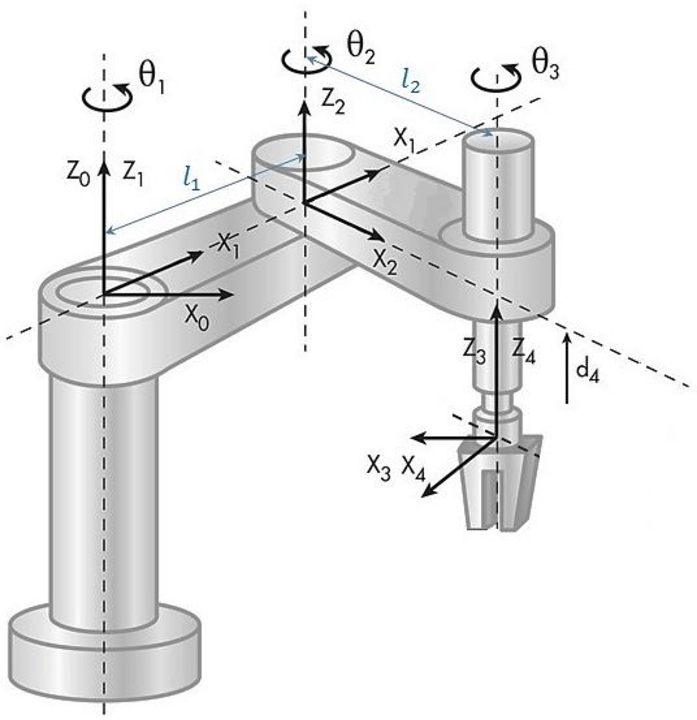
\includegraphics[width=0.5\textwidth]{SCARA-robot-of-4-gdl-Source-Our-elaboration.png}
\caption{SCARA type manipulator. }
\end{figure}

What is the workspace volume for this robot?. (Draw a picture of it as well)
\part[5] Write the DH parameters 
\part[10] Compute the forward kinematics to find the position of the end effector if $\theta_1 = 30 deg$, $\theta_2 = 45 deg$, $\theta_3 = 90 deg$, and $d = 14 cm$

\end{parts}



\newpage

\addpoints
\question[20]

Inverse Kinematics with numerical approaches

\noaddpoints
\begin{parts}



\part[10] Compute the joint angles and extension distances that will get this robot to pick up an object at x=1.2, y=0.8, z=0.5
\begin{figure}
\centering
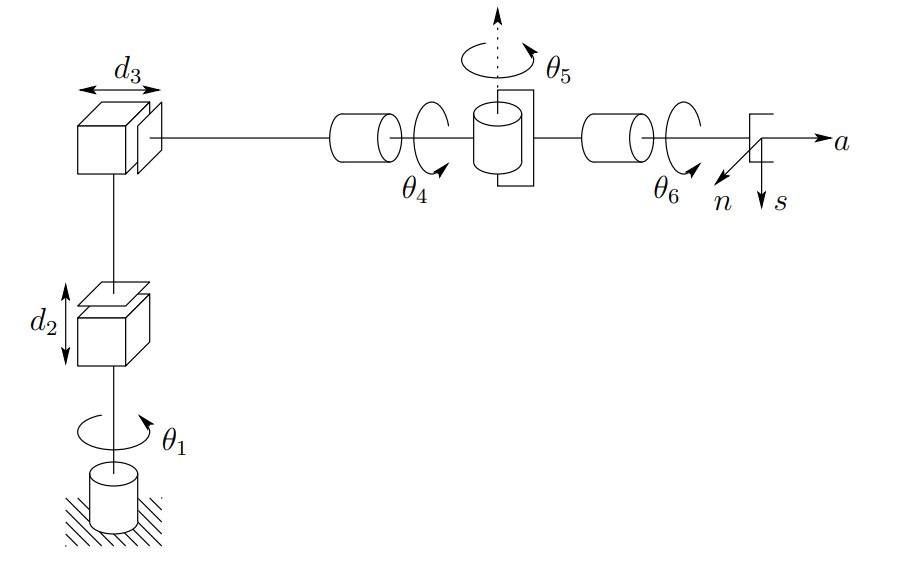
\includegraphics[width=0.5\textwidth]{6dof_arm.jpg}
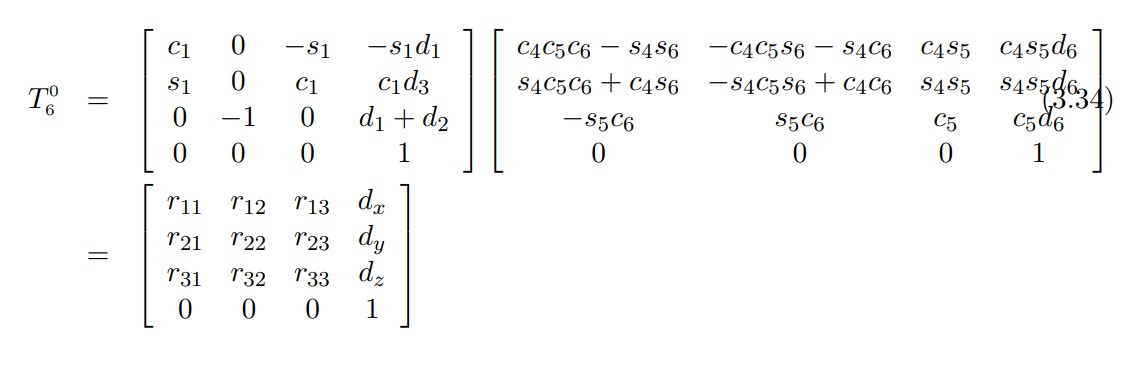
\includegraphics[]{6dof_arm_TMatrix.jpg}
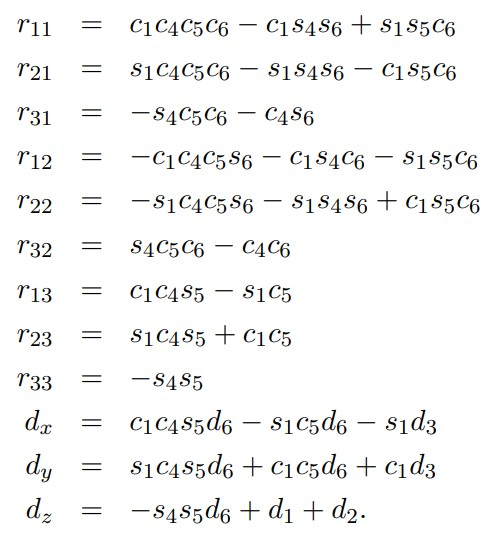
\includegraphics[]{6dof_arm_TMatrix_Eqs.jpg}
\caption{Cylindrical/Prismatic manipulator. Use for problem 6.}
\end{figure}


\part[10] What would be the joint angles and extension distances to get to the same goal coordinates if the robot started with the end effector at $\theta_1= -90deg$, $d_2 = 0.5m$, $d_3 = 1.0m$, $\theta_4=-90deg$, $\theta_5 = 90deg$, $\theta_6 = 40deg$ and we wished to minimize the total distance traveled for each actuating part?

\end{parts}

\newpage

\addpoints
\question[20]

Energy Optimal Manipulation

\noaddpoints
\begin{parts}

\part[10] Using the same system, start configuration, and goal coordinates as in question 5, compute the energy efficient joint angles and extension distances. For your energy model, assume that actuating $\theta_1$ costs 3x the energy of $\theta_{4,5,6}$, and $d_{2,3}$ costs 2x the energy.

\part[10] There are two locations you need to reach, one at $ (1, 1, 1)$ and the other at $(-1, 2, 1$. Which would you go to first and how much energy will you expend in your overall task?

\end{parts}


\newpage

\addpoints
\question[20]
Human Emotions

\noaddpoints
\begin{parts}

\part[10] Using the FER library in python, example in the following link:  \url{https://towardsdatascience.com/the-ultimate-guide-to-emotion-recognition-from-facial-expressions-using-python-64e58d4324ff}
build a system that classifies human emotions and validate on video 1 and 2 from this repository: \url{https://github.com/rjrahul24/ai-with-python-series/tree/main/07.%20Emotion%20Recognition%20using%20Live%20Video}
Generate plots of predicted emotions over time for both videos.

\part[10] What are the logical applications of this tool for an autonomous robot? What are the ethical and legal consequences of fielding a system that makes decisions based on this tool?

\end{parts}



\newpage

\addpoints
\question[20]
Motion Planning


\noaddpoints
\begin{parts}

\part[10] Using one of the planners found in \url{https://github.com/AtsushiSakai/PythonRobotics/tree/master/PathPlanning}, implement a planner for any generic robot and compare the performance against Djikstra, A star, and RRT star.

\part[10] Implement a skid-steer (4 wheel) vehicle model for a robot 33 inches wide, by 40 inches long for the planner that you chose.

\end{parts}




\newpage

\addpoints
\question[20]
Object Detection (Please put the classified images as part of your submission)

\noaddpoints
\begin{parts}
\part[5] Classify the first 5 pictures in \url{https://www.tensorflow.org/datasets/catalog/sun397} using any image classification algorithm.

\part[5] Implement Yolo and do the same, what are the differences. 

\part[10] Using transfer learning, pick an image classification algorithm and retrain it to learn to detect a new object of interest.

\end{parts}




\newpage

\addpoints
\question[20]
Ethics of Robotics - Open Ended Questions

\noaddpoints
\begin{parts}

\part[5] Many people (particularly those in the robotics industry) believe that robotics is purely within the purview of technical development and should not have any ethical considerations. What do you feel can be a merit or demerit to this way of thinking?

\part[5] Isaac Asimov listed 3 laws of robotics, comment on the algorithmic complexity of implementing these into working intelligence. 

\part[5] In the event of an autonomous system causing harm or damages, who is responsible? 

\part[5] What laws may be helpful for regulating or controlling autonomous systems? What drawbacks will this potentially have?

\end{parts}



% You are tasked with surveying a remote agricultural area in Cote d'Ivoire which produces cocoa beans for top chocolate makers (yay chocolate!). Because of the costs of operation in this region of the world, you have been tasked with getting a robot to move from a base-station to survey a small patch of cocoa trees and estimate crop yeilds. 

% \noaddpoints
% \begin{parts}
% \part[5] What is the state space of the problem? What are the critical pieces of information that you feel is relevant to solving the problem? Are there any assumptions you are making in being able to access this information? Write this as a list, ie: State = ['something1', 'something2', ect.], assumptions = ['none', 'heroic assumption about amazing sensor', ect.]

% \part[10] Write your cost function? Does it have units? (If yes, what are they?) What are you penalizing/rewarding? Write this in the form of: Cost = <function>

% \part[10] What is a good heuristic function that can estimate your cost to accomplish this objective? (Note that this should be in the same units as your cost function.) What are the drawbacks and simplifications this function is making?

% \part[15] 
% What would your search algorithm look like? Illustrate the logic your system would follow to make a crop yeild estimate. (Draw a diagram of a few trees, where would your robot go first, how does your cost and heuristic fit together?) How much would you trust this information in making decisions about moving labor and resources here?


% \end{parts}

% \fillwithdottedlines{8em}

\end{questions}

\end{document}
